This component receives the answers of the Question-Answering system, interprets them and outputs \textit{tokens for predictions}.
% stemming
\subsection{Stemming}
\label{sec:stemming}
Before the interpretation, the answers are stemmed using the \textit{Snowball Stemmer} present in NLTK with a slight modification. This because it is true that stemming reduces the variability of text, mapping inflected or derived words into their root form (the stem); but it is also true that a stem need not be identical to the morphological word root. This is a problem because a stemmer might output out-of-vocabulary words, which cannot be vectorified. Thus, the solution to this problem stands in accepting the stemmed word only if it is inside the vocabulary (the list of the first $100\,000$ terms in GloVe pre-trained embeddings). This stemmer is also used in the calculation of the representative embeddings of symptoms (which will be discussed later).

\subsection{Filtering ``unuseful words''}
The stemmed answers are then passed to a function that filters ``unuseful words''. Basically, this function keeps only words that are tagged as a \textit{part of speech} that is inside the following list: noun, adjective, coordinating conjunction, punctuation, verb and auxiliar. For this purpose I used the Stanford POS Tagger, which is inside Stanford NLP library. Thus, the basic idea is to simplify the answer deleting words like adverbs and pronouns that do not contribute to the meaning of the symptoms.

\subsection{Answer interpretation}
The two different types of answers are processed in a different way:
\begin{itemize}
  \item the general answer about symptoms is one for each passage. Usually, this answer contains more symptoms separated by a coordinating conjunction (mainly, comma and ``and''). For this reason, the Answer Interpreter splits the answer on these particles and originates one or more \textit{tokens for predictions}.
  \item the specific answers about a body part are as many as the number of body parts found in the passage. Given a body-part answer, the \textit{token for prediction} is formed concatenating the answer with the name of the body part.
\end{itemize}

\begin{figure}[h]
\centering
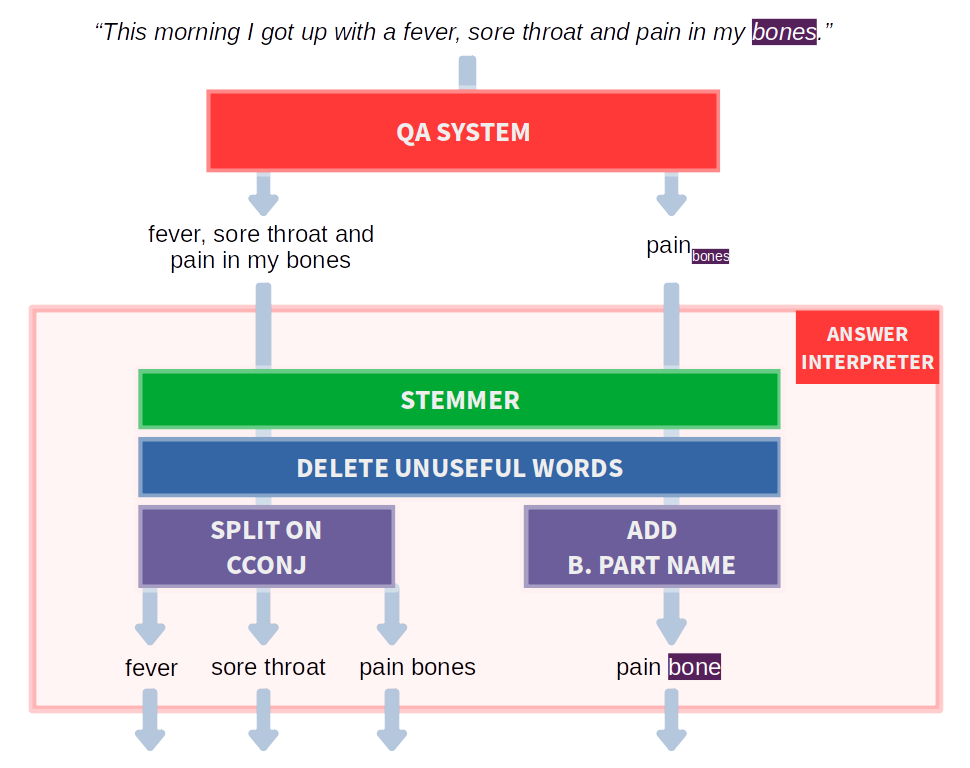
\includegraphics[width=13cm]{answer_interpreter}
\caption{The Answer Interpreter illustrated}
\medskip
\label{fig:answer_int}
\end{figure}
